%%%% Better Poster latex template example v1.0 (2019/04/04)
%%%% GNU General Public License v3.0
%%%% Rafael Bailo
%%%% https://github.com/rafaelbailo/betterposter-latex-template
%%%% 
%%%% Original design from Mike Morrison
%%%% https://twitter.com/mikemorrison

\documentclass[a0paper,fleqn]{betterposter}

% For gt table latex
\usepackage{amsmath, booktabs, caption, longtable}

\usepackage{fontawesome}
\usepackage{xcolor}

% For custom lists
\renewcommand{\labelenumii}{\arabic{enumi}.\arabic{enumii}}
\renewcommand{\labelenumiii}{\arabic{enumi}.\arabic{enumii}.\arabic{enumiii}}
\renewcommand{\labelenumiv}{\arabic{enumi}.\arabic{enumii}.\arabic{enumiii}.\arabic{enumiv}}

% Font awesome symbols https://mirrors.ibiblio.org/CTAN/fonts/fontawesome/doc/fontawesome.pdf

%%%% Uncomment the following commands to customise the format

%% Setting the width of columns
% Left column
% \setlength{\leftbarwidth}{0.22\paperwidth}
% Right column
%\setlength{\rightbarwidth}{0.25\paperwidth}

%% Setting the column margins
% Horizontal margin
%\setlength{\columnmarginvertical}{0.05\paperheight}
% Vertical margin
%\setlength{\columnmarginhorizontal}{0.05\paperheight}
% Horizontal margin for the main column
%\setlength{\maincolumnmarginvertical}{0.15\paperheight}
% Vertical margin for the main column
%\setlength{\maincolumnmarginhorizontal}{0.15\paperheight}

%% Changing font sizes
% Text font
\renewcommand{\fontsizestandard}{\fontsize{28}{50} \selectfont}
% Main column font
\renewcommand{\fontsizemain}{\fontsize{115}{150} \selectfont}
% Title font
% \renewcommand{\fontsizetitle}{\fontsize{68}{150} \selectfont}
% Author font
\renewcommand{\fontsizeauthor}{\fontsize{40}{50} \selectfont}
% Section font
%\renewcommand{\fontsizesection}{\fontsize{28}{35} \selectfont}

%% Changing font sizes for a specific text segment
% Place the text inside brackets:
% {\fontsize{28}{35} \selectfont Your text goes here}
% \definecolor{Mycolor2}{HTML}{C17C74}
\definecolor{Mycolor2}{HTML}{6C91C2} 
%% Changing colours
% Background of side columns
%\renewcommand{\columnbackgroundcolor}{black}
% Font of side columns
%\renewcommand{\columnfontcolor}{gray}
% Background of main column
\renewcommand{\maincolumnbackgroundcolor}{Mycolor2}
%\renewcommand{\maincolumnbackgroundcolor}{theory}
%\renewcommand{\maincolumnbackgroundcolor}{methods}
%\renewcommand{\maincolumnbackgroundcolor}{intervention}
% Font of main column
%\renewcommand{\maincolumnfontcolor}{gray}

\begin{document}	
\betterposter{
%%%%%%%% MAIN COLUMN

\maincolumn{
%%%% Main space
\vspace{-1in}
\textbf{iNaturalist} data informs \\regional \textbf{conservation} strategy
\vspace{-3in}


% \begin{figure}[!tbp]
  \centering
  \begin{minipage}[t]{0.3\textwidth}
    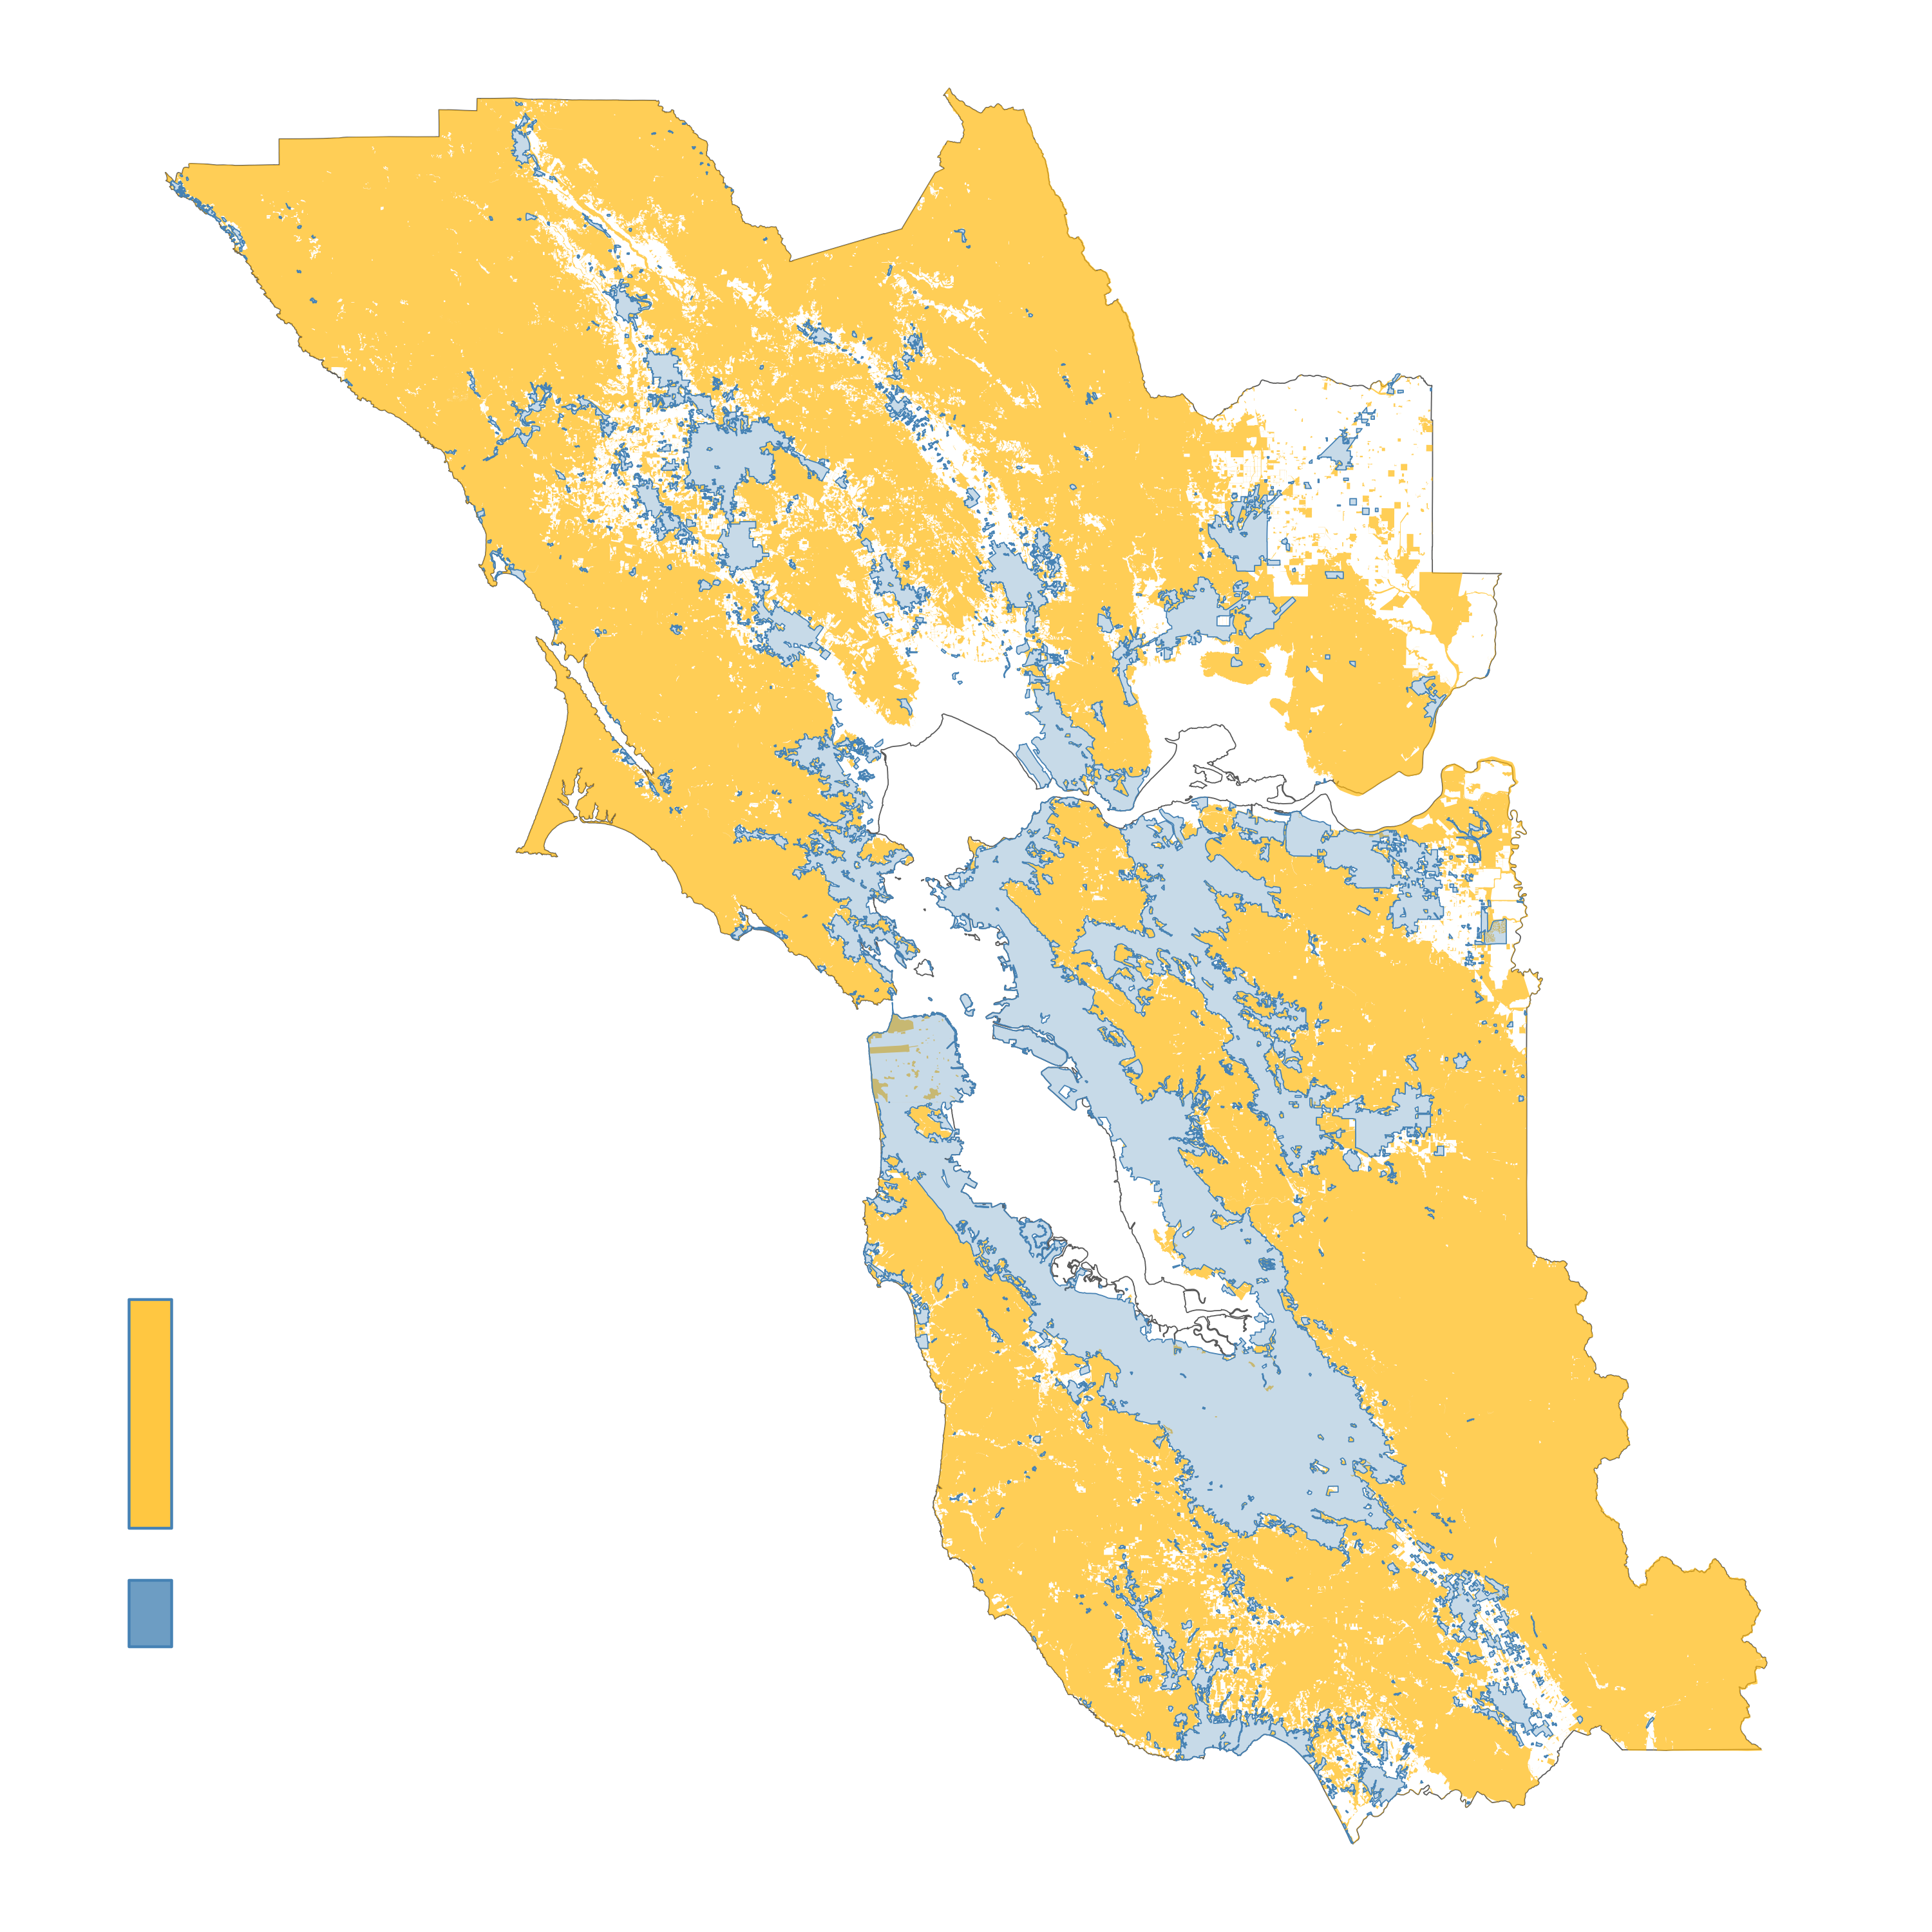
\includegraphics[width=\textwidth]{img/urbancln.png}
  \end{minipage}
  \hfill
  \begin{minipage}[c]{0.65\textwidth}
  \vspace{9in}
    % 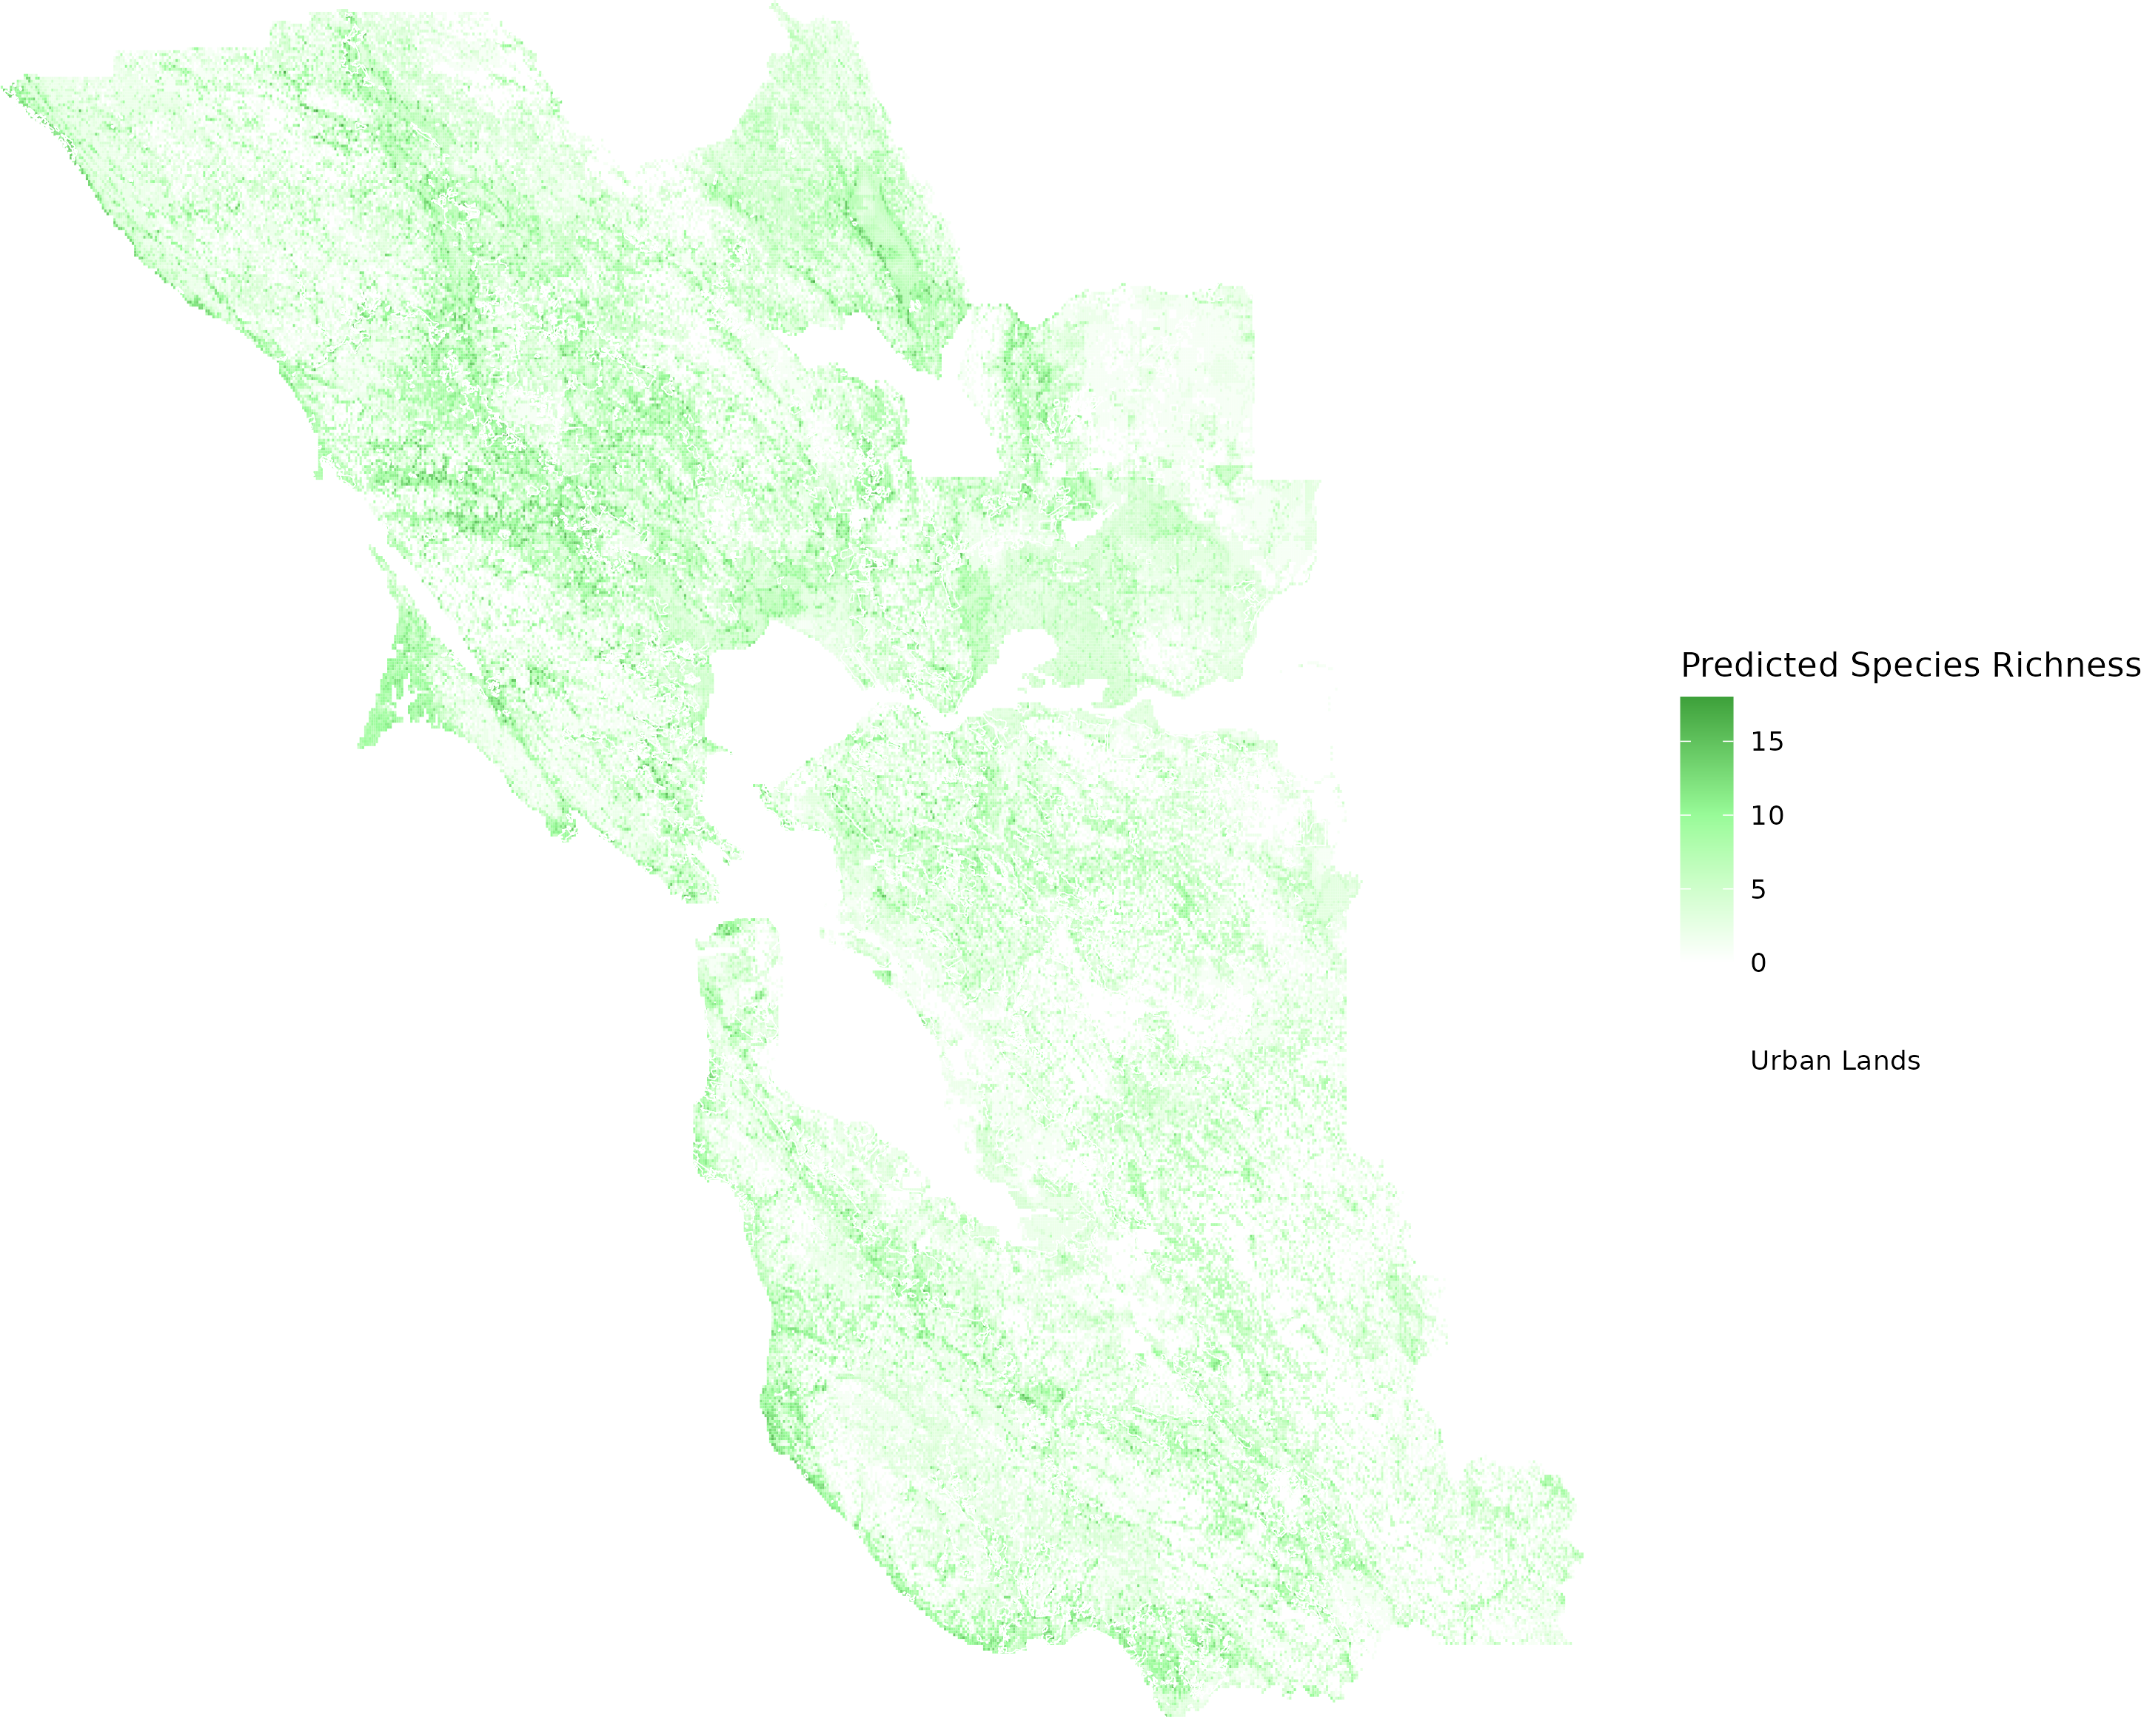
\includegraphics[width=\textwidth]{img/species_richness.png}
    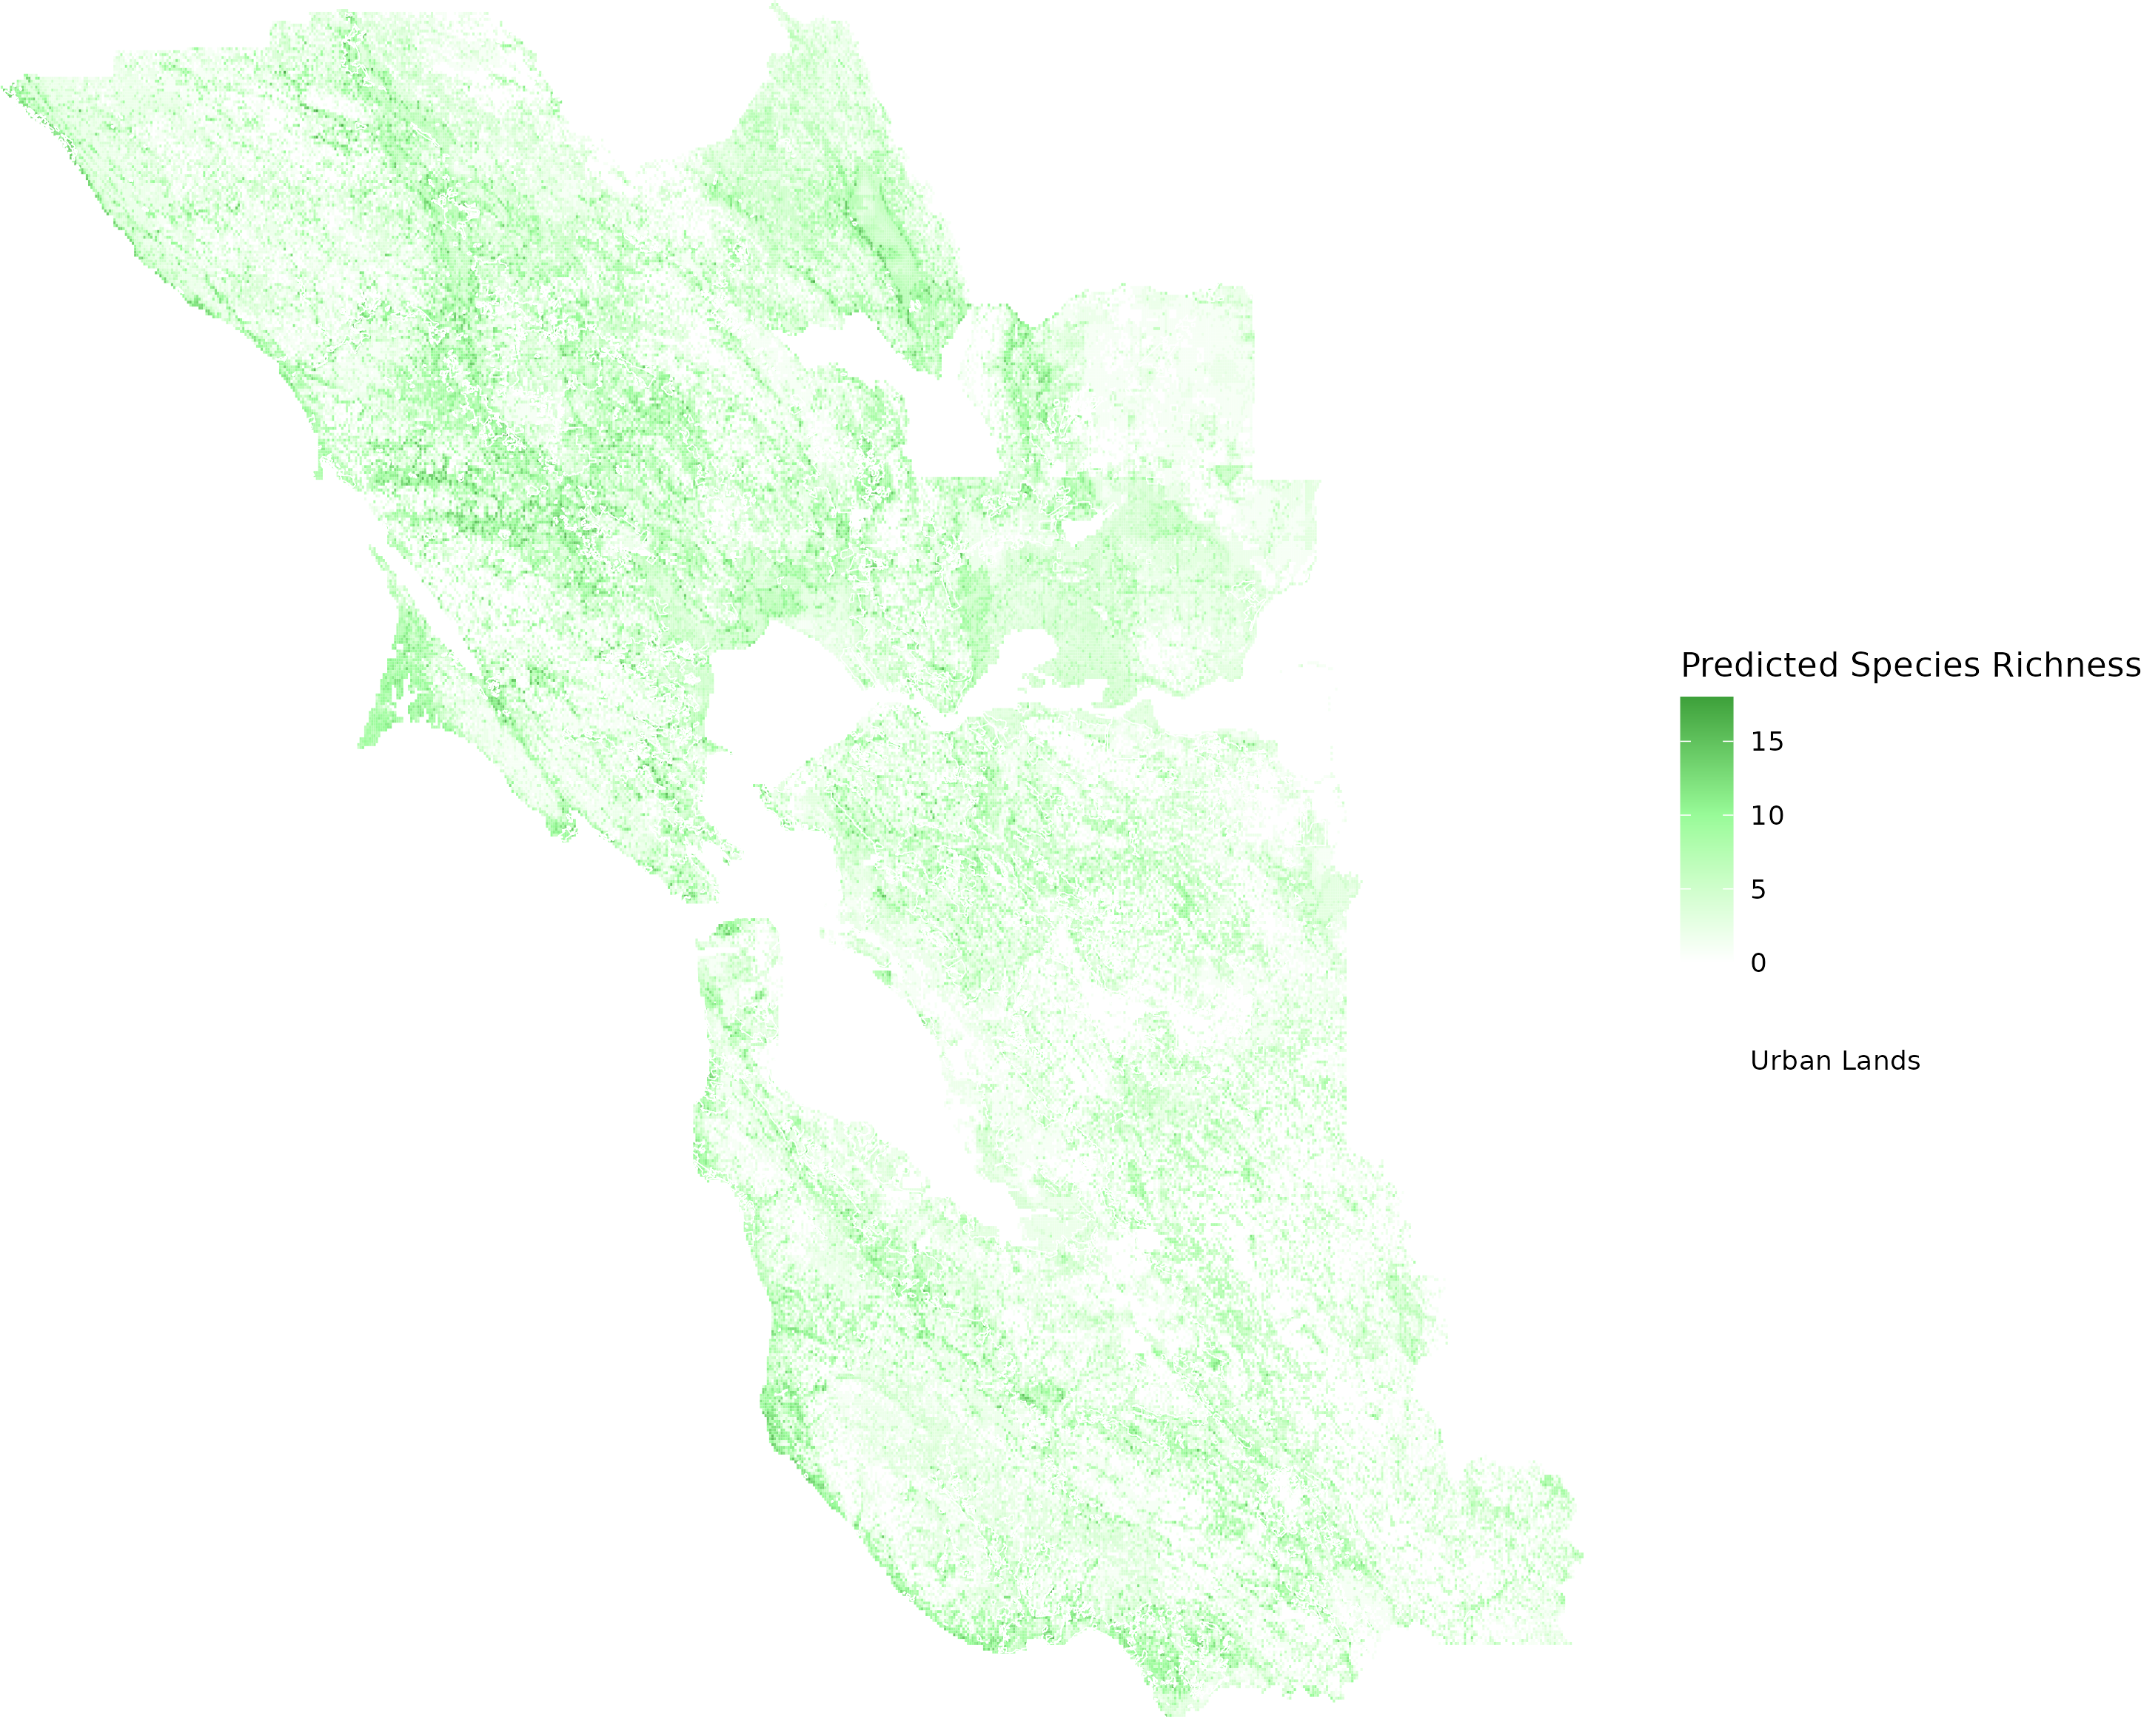
\includegraphics[width=\textwidth]{img/species_richness.eps}
  \end{minipage}
% \end{figure}
% 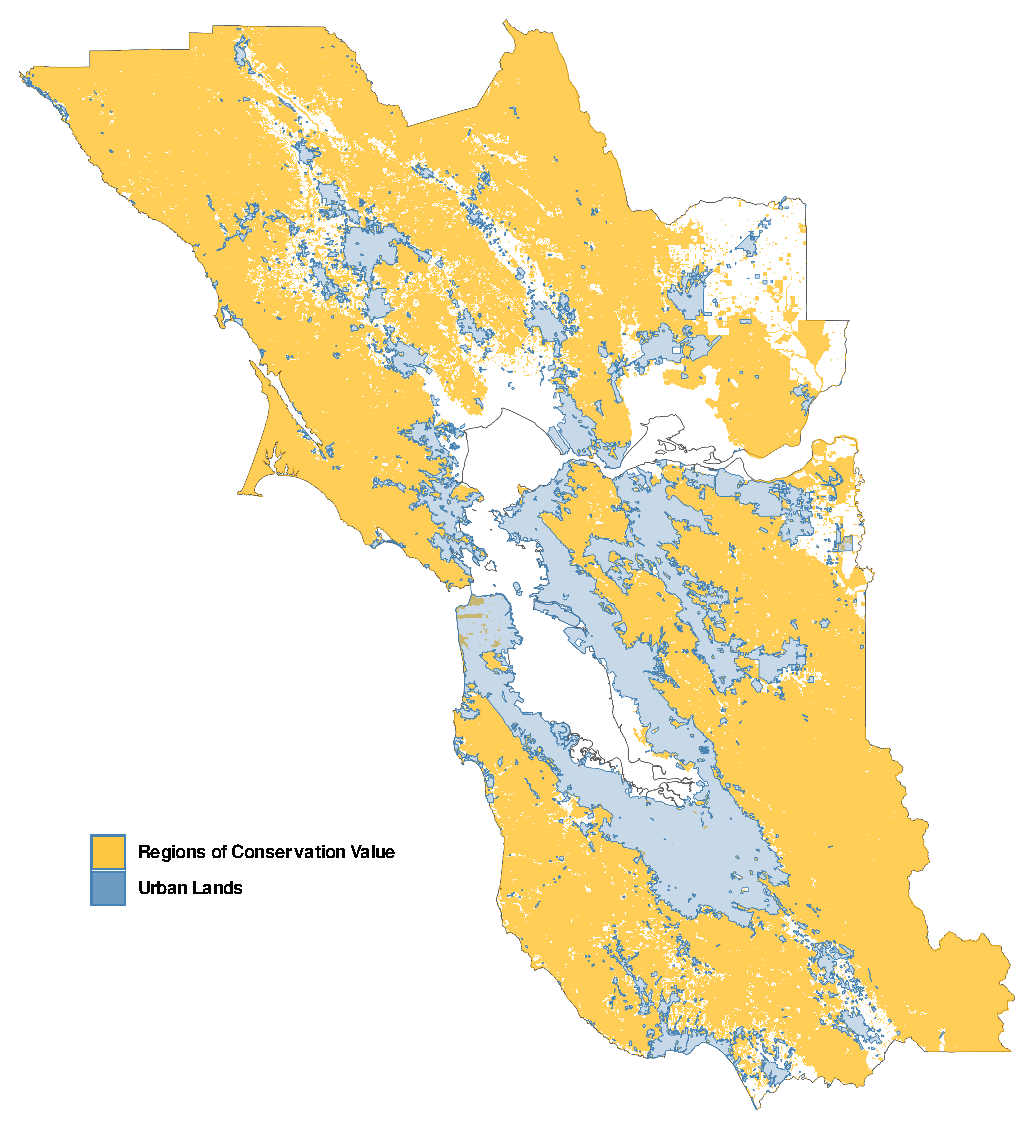
\includegraphics[width=.3\textwidth]{img/urbancln.eps}

% 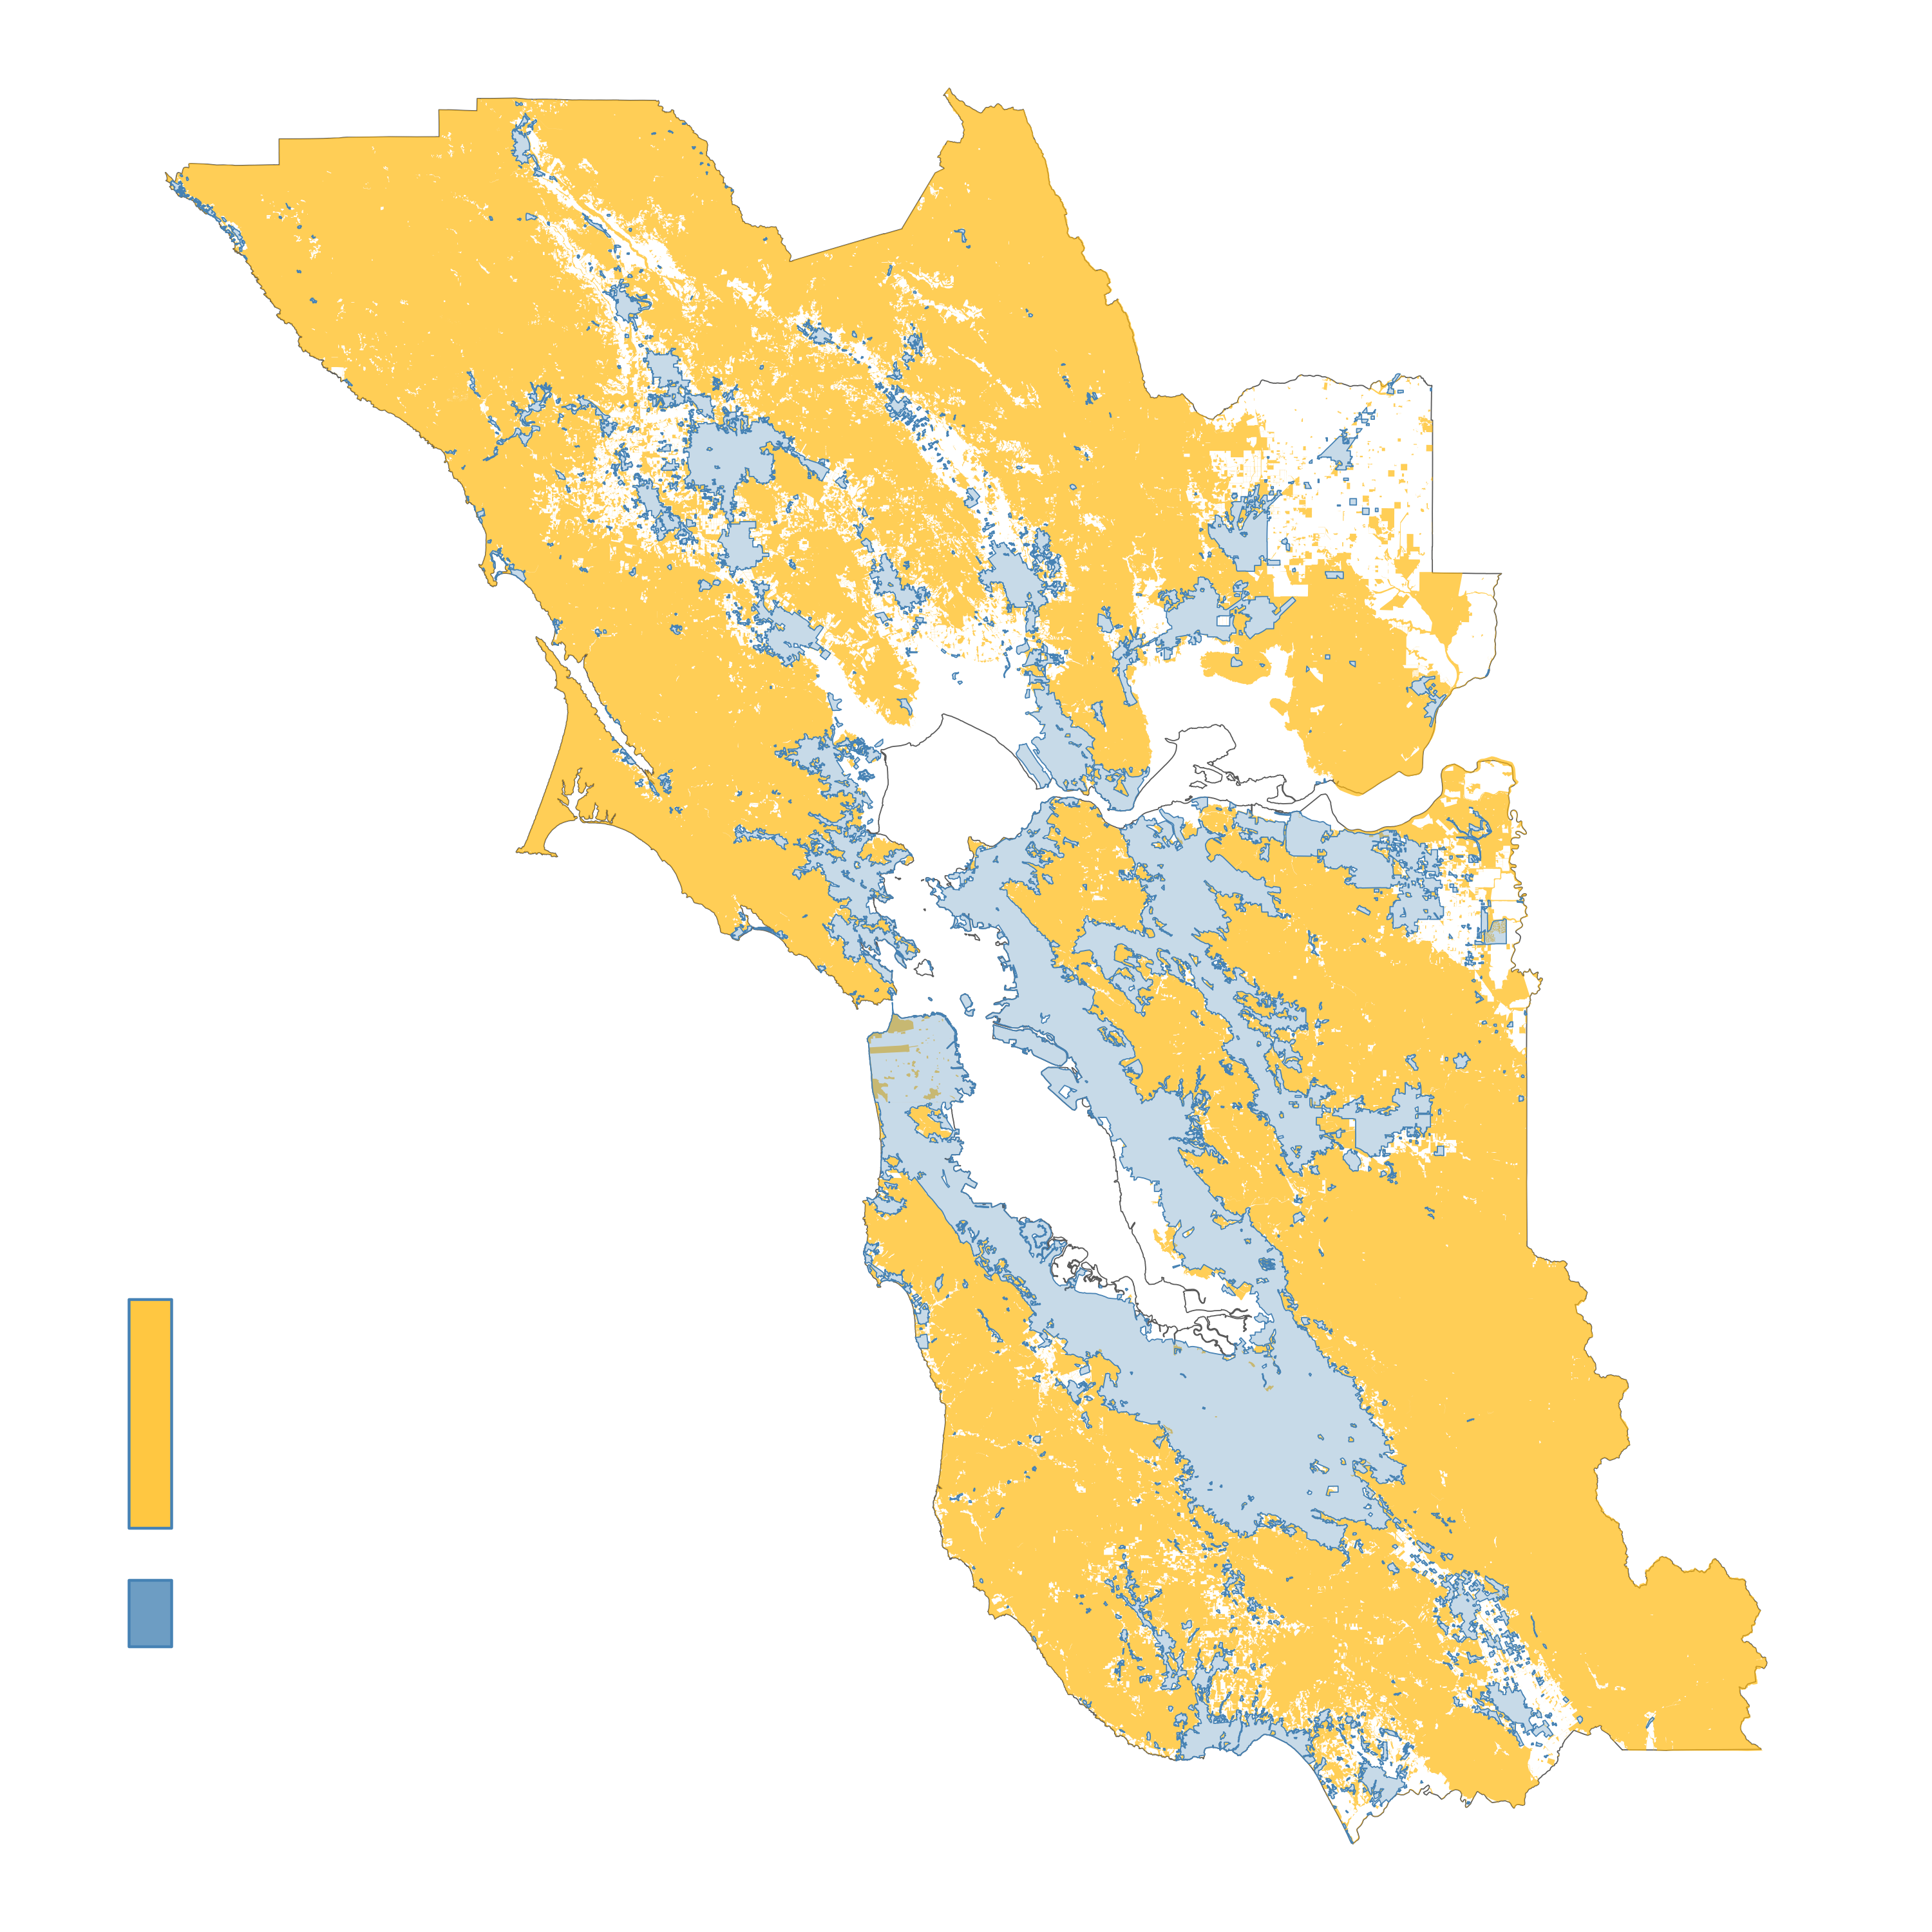
\includegraphics[width=.3\textwidth]{img/urbancln.png}
% 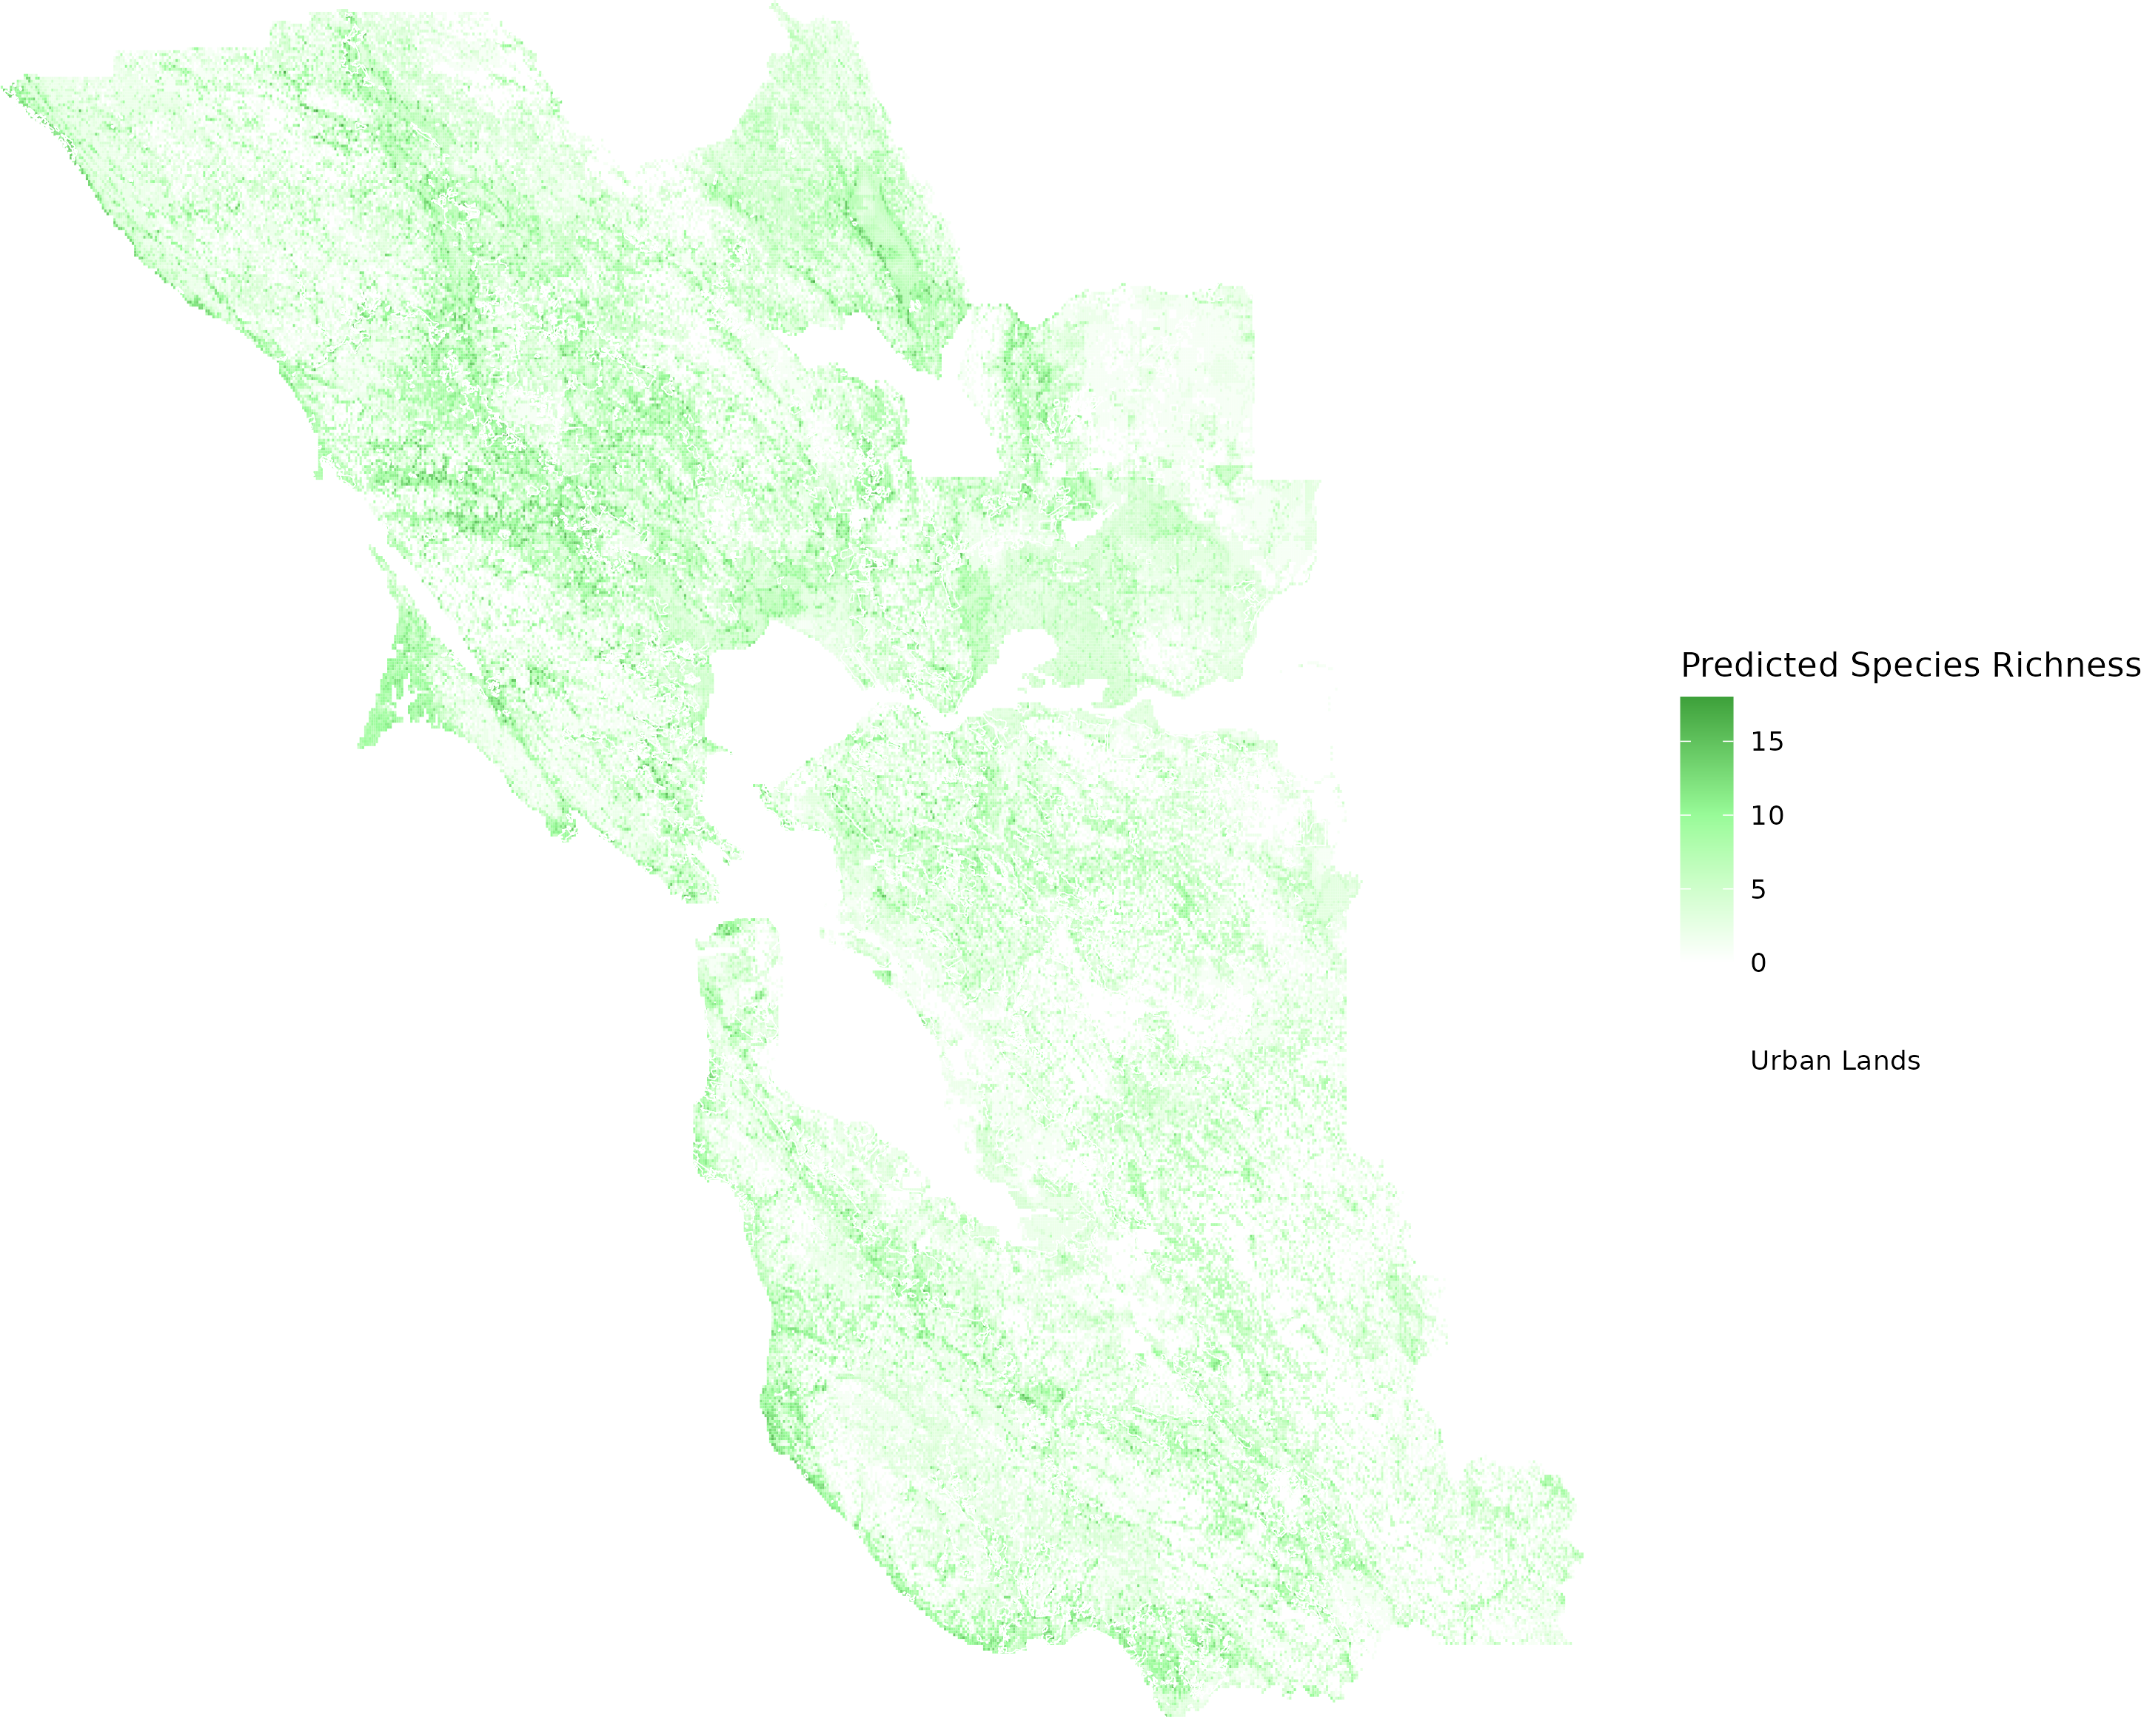
\includegraphics[width=.65\textwidth]{img/species_richness.eps}
% \\\textbf{Emphasize} the important words.
% \vfill
}{
%%%% Bottom space

%% QR code
\vspace{-4in}
\qrcode{img/qr-code}{img/smartphoneWhite}{
\textbf{Scan the QR code} to
\\view the interactive report
\\we sent to community collaborators
}
% Smartphone icon
% Author: Freepik
% Retrieved from: https://www.flaticon.com/free-icon/smartphone_65680

}

}{
%%%%%%%% LEFT COLUMN

\title{Evaluating the contribution of urban lands to SF Bay Area conservation goals with iNaturalist}
\author{Avery Hill$^1$, Tom Robinson$^2$, Rebecca Johnson$^1$, Alison Young$^1$}

\institution{$^1$California Academy of Sciences}

\institution{$^2$Together Bay Area}

\section{Introduction}

\vspace{-2cm}
\begin{itemize}
\item Regional \textbf{conservation} organizations in the San Francisco Bay Area have \textbf{not yet recognized} the extent to which \textbf{urban lands} provide habitat for target conservation species.
\item The biodiversity community science platform, \textbf{iNaturalist}, demonstrates that many \textbf{target species} are \textbf{frequently observed} in urban landscapes.
\item \textbf{Species distribution modeling} (SDM) is a powerful tool for evaluating the habitat of target species and mapping available habitat across urban areas.
\end{itemize}

\section{Materials}
% We trained SDMs for X species using regional iNaturalist observations and X environmental variables.
% \vspace{1cm}
% \fontsize{15}{15}
\def\iconspace{2mm}
\vspace{-15mm}
\\\faMapO   \hspace{1cm} 10 San Francisco Bay Area counties
\vspace{\iconspace}
\\\faClockO \hspace{1cm} 1999 - 2023
\vspace{\iconspace}
\\\faMapMarker \hspace{1.3cm} 53,000 iNaturalist observations
\vspace{\iconspace}
\\\faLeaf \hspace{1cm} 18 species of conservation value
\vspace{\iconspace}
\\\faSunO \hspace{.9cm} 18 environmental variables at 10m
% \vspace{\iconspace}
% \\\faConnectdevelop \hspace{1cm} Maxent SDM, 5-fold cross validation
\vspace{\iconspace}
\\\faCode \hspace{1cm} R v4.2.2, \textit{SDMTune}, \textit{blockCV}, \textit{terra}, 
\\ \hspace*{2.1cm} \textit{tidyverse}, \textit{CoordinateCleaner}, \textit{sf}
% \begin{center}


\section{Methods}
% % \includegraphics[width=\textwidth]{img/tikzexample1}
% \end{center}
\vspace{-15mm}
% {\fontsize{31}{45} \selectfont
\begin{enumerate}
    \item Prepare source data
    % \begin{enumerate}
    %     \item Clean iNaturalist observations
    %     \item Standardize environmental variables 
    % \end{enumerate}
    \item Train MaxEnt SDM for each species
    % \begin{enumerate}
    %     \item Separate train and test sets
    % \end{enumerate}
    \item Validate models with local experts
    \item Identify important habitat for target species
\end{enumerate}
% }




}{
%%%%%%%% RIGHT COLUMN
\section{Extended Results}

\textbf{Species with SDM Accuracy Metrics}
\begingroup % localize the following settings                                                                    
% \setlength\tabcolsep{2pt}
% \footnotesize
% \fontsize{10}{10}
\huge
% \centering
% \setlength\LTcapwidth{\textwidth} % default: 4in (rather less than \textwidth...)      

% \setlength\LTleft{0pt}            % default: \fill
% \setlength\LTright{0pt}           % default: \fill
\begin{longtable}{l|rrr}
\toprule
\multicolumn{1}{l}{} & Presence Points & AUC & TSS \\ 
\midrule
Aneides lugubris & 1815 & 0.82 & 0.48 \\ 
Aphelocoma californica & 5902 & 0.79 & 0.42 \\ 
Callipepla californica & 2952 & 0.86 & 0.56 \\ 
Canis latrans & 3354 & 0.86 & 0.54 \\ 
Chlorogalum pomeridianum & 3873 & 0.85 & 0.52 \\ 
Danaus plexippus & 3904 & 0.90 & 0.64 \\ 
Elgaria coerulea & 506 & 0.93 & 0.71 \\ 
Elgaria multicarinata & 1809 & 0.79 & 0.43 \\ 
Helminthoglypta nickliniana & 155 & 0.95 & 0.77 \\ 
Juglans hindsii & 81 & 0.94 & 0.73 \\ 
Lontra canadensis & 602 & 0.98 & 0.85 \\ 
Melanerpes formicivorus & 4116 & 0.86 & 0.56 \\ 
Nycticorax nycticorax & 3346 & 0.96 & 0.78 \\ 
Sciurus griseus & 1375 & 0.92 & 0.68 \\ 
Sialia mexicana & 5075 & 0.84 & 0.51 \\ 
Thamnophis elegans & 308 & 0.91 & 0.66 \\ 
Thamnophis sirtalis & 38 & 0.97 & 0.86 \\ 
Zonotrichia leucophrys & 5198 & 0.89 & 0.63 \\ 
\bottomrule
\end{longtable}

 
\endgroup

\vspace{1in}
\textbf{Most Important Environmental Variables}
\begin{center}
    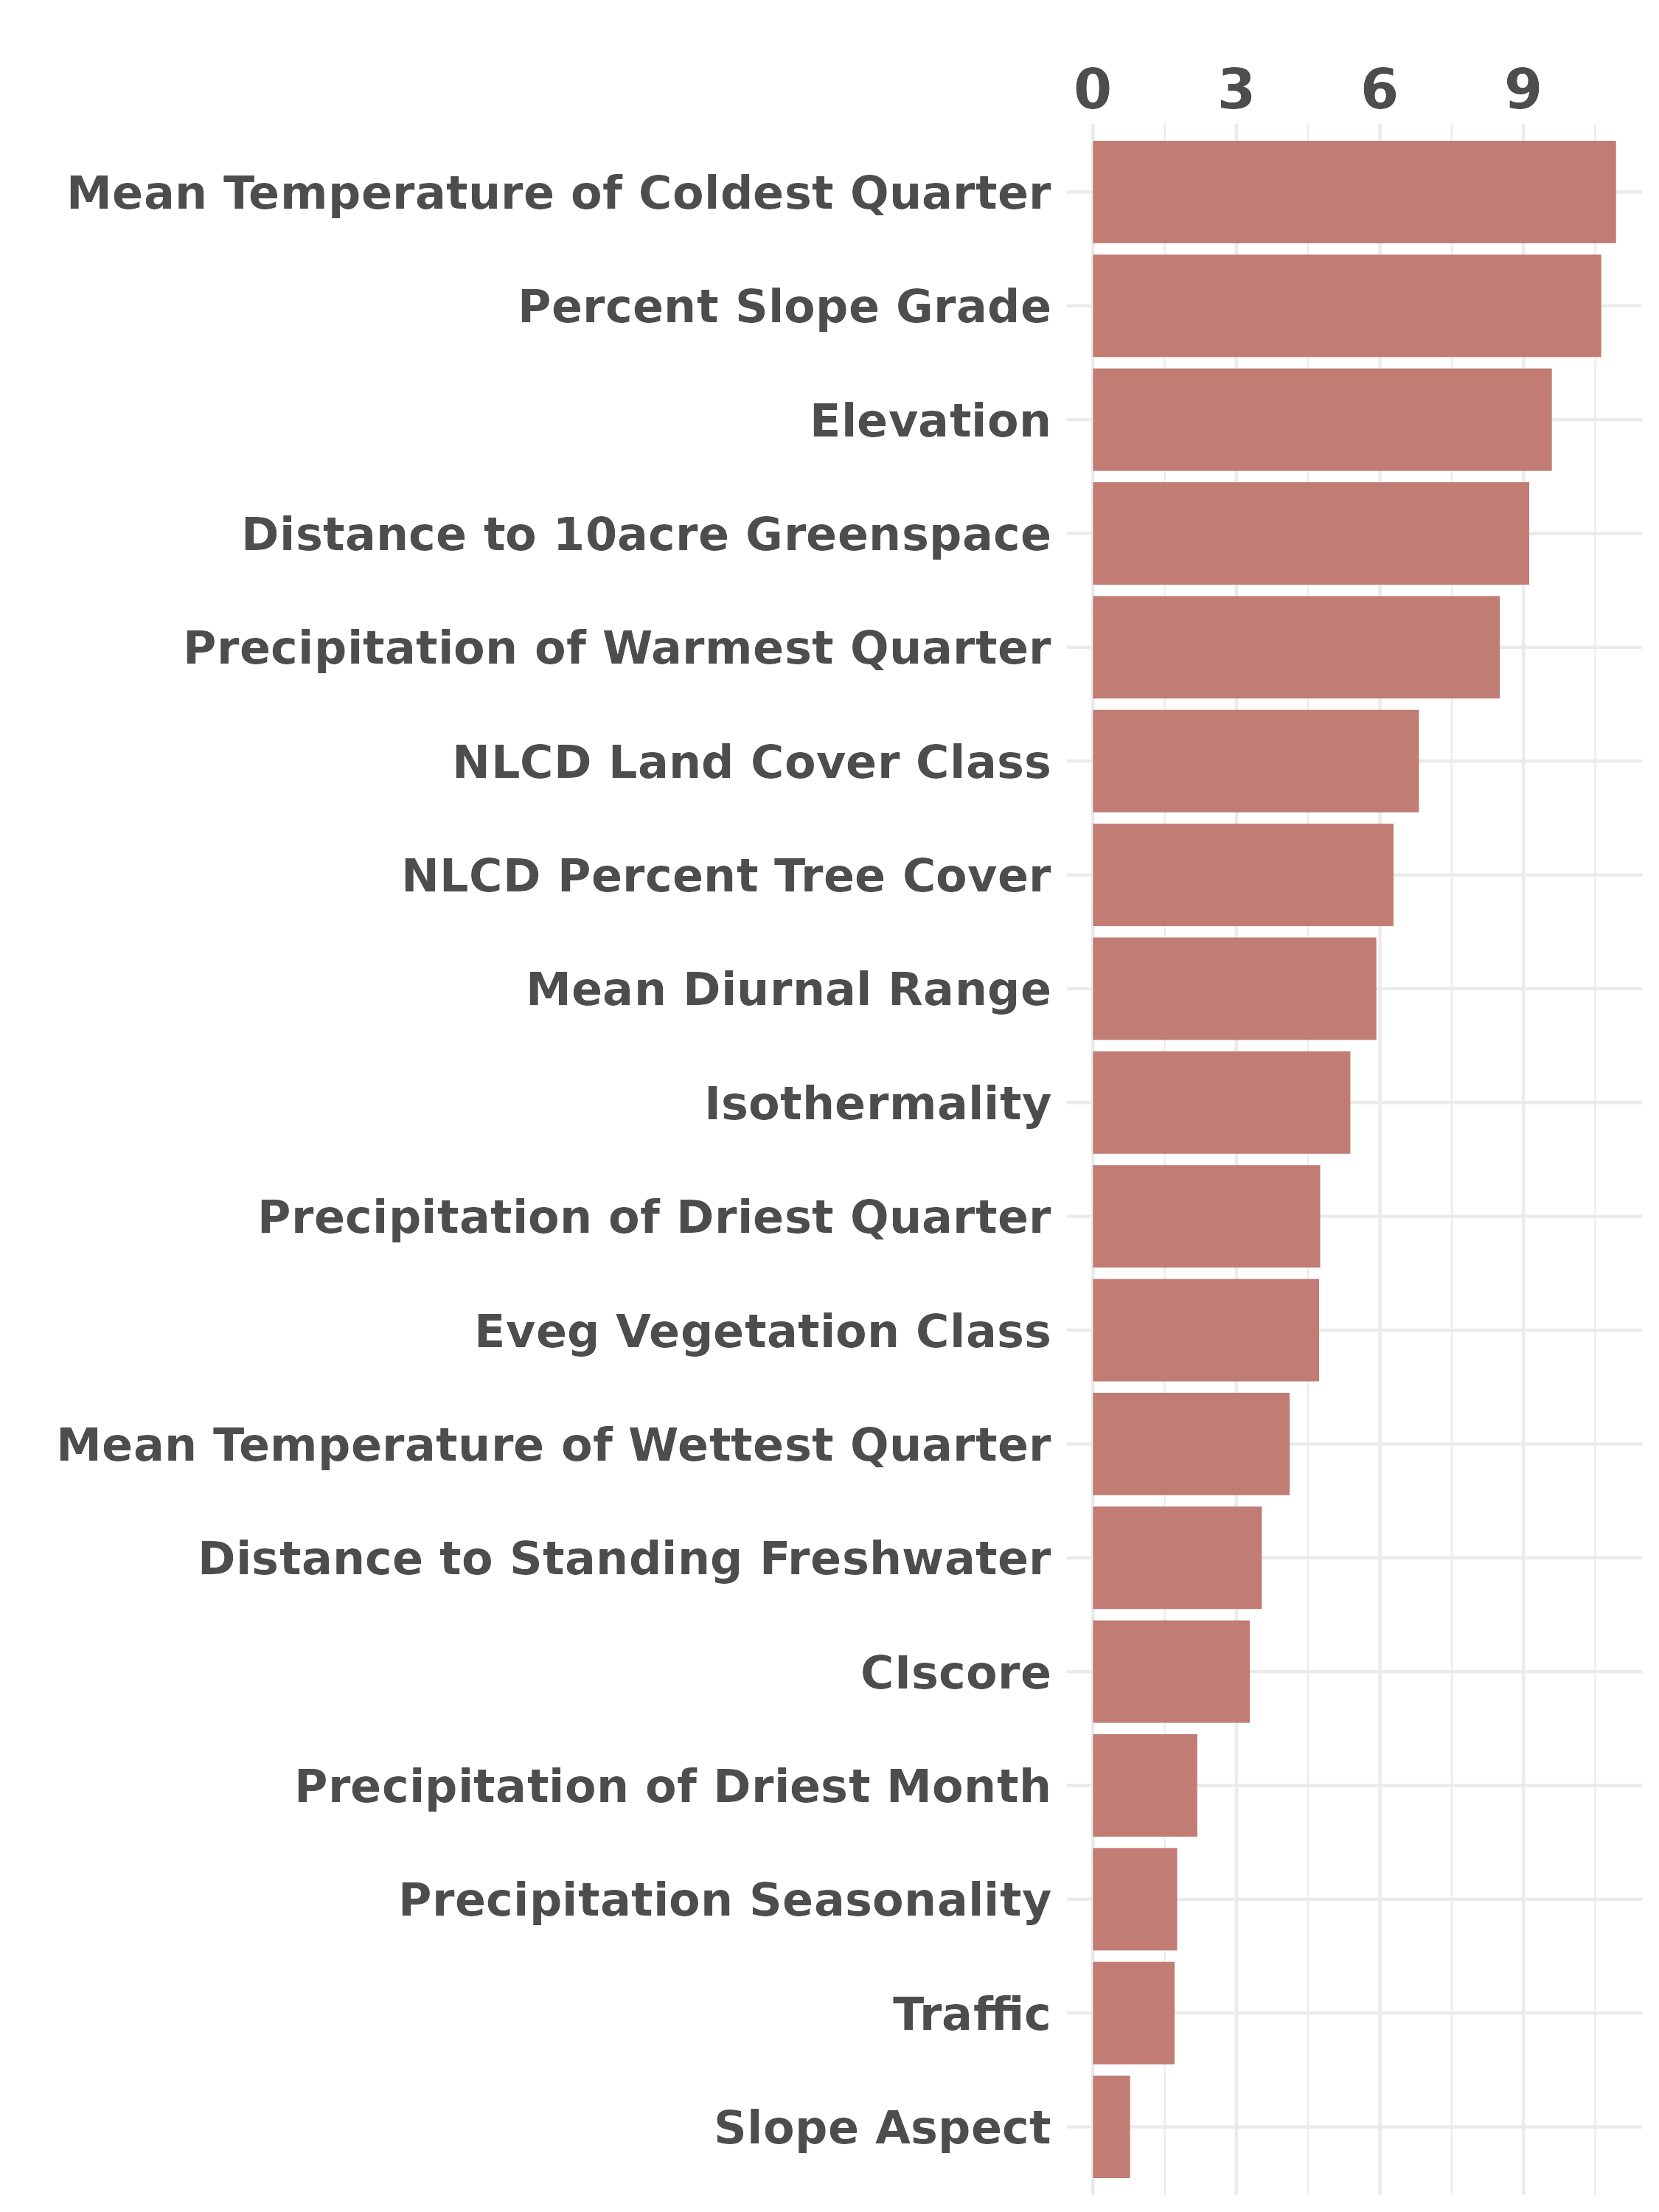
\includegraphics[width = \textwidth]{img/predictor.png}
\end{center}

\vspace{1cm}
\section{Conclusion}
\vspace{-1cm}
\begin{itemize}
\item iNaturalist and accessible environmental data can produce informative SDMs
\item Many target conservation species in the Bay Area find habitat in urban landscapes
\end{itemize}

\vfill

%% Institution logo
\begin{center}


\includegraphics[width=.8\textwidth]{img/combined_logo.eps}\\
% \end{right}
\end{center}
}
\end{document}
